\setchapterpreamble[u]{\margintoc}
\chapter{Summary of published results}
\label{ch:summary}

This part of the document reproduces five articles published in peer-reviewed journals authored by the candidate. They represent the core contributions of the present thesis. However, there are many more outcomes resulting from the research work produced during the course of the doctoral studies. These include other journal articles co-authored in collaboration with other colleagues in tangential topics, national and international conferences, disseminative talks in seminars, several software libraries and one book. \autoref{fig:dashboard} indicates the main numbers related to the different types of works developed.

\begin{figure*}[htbp]
    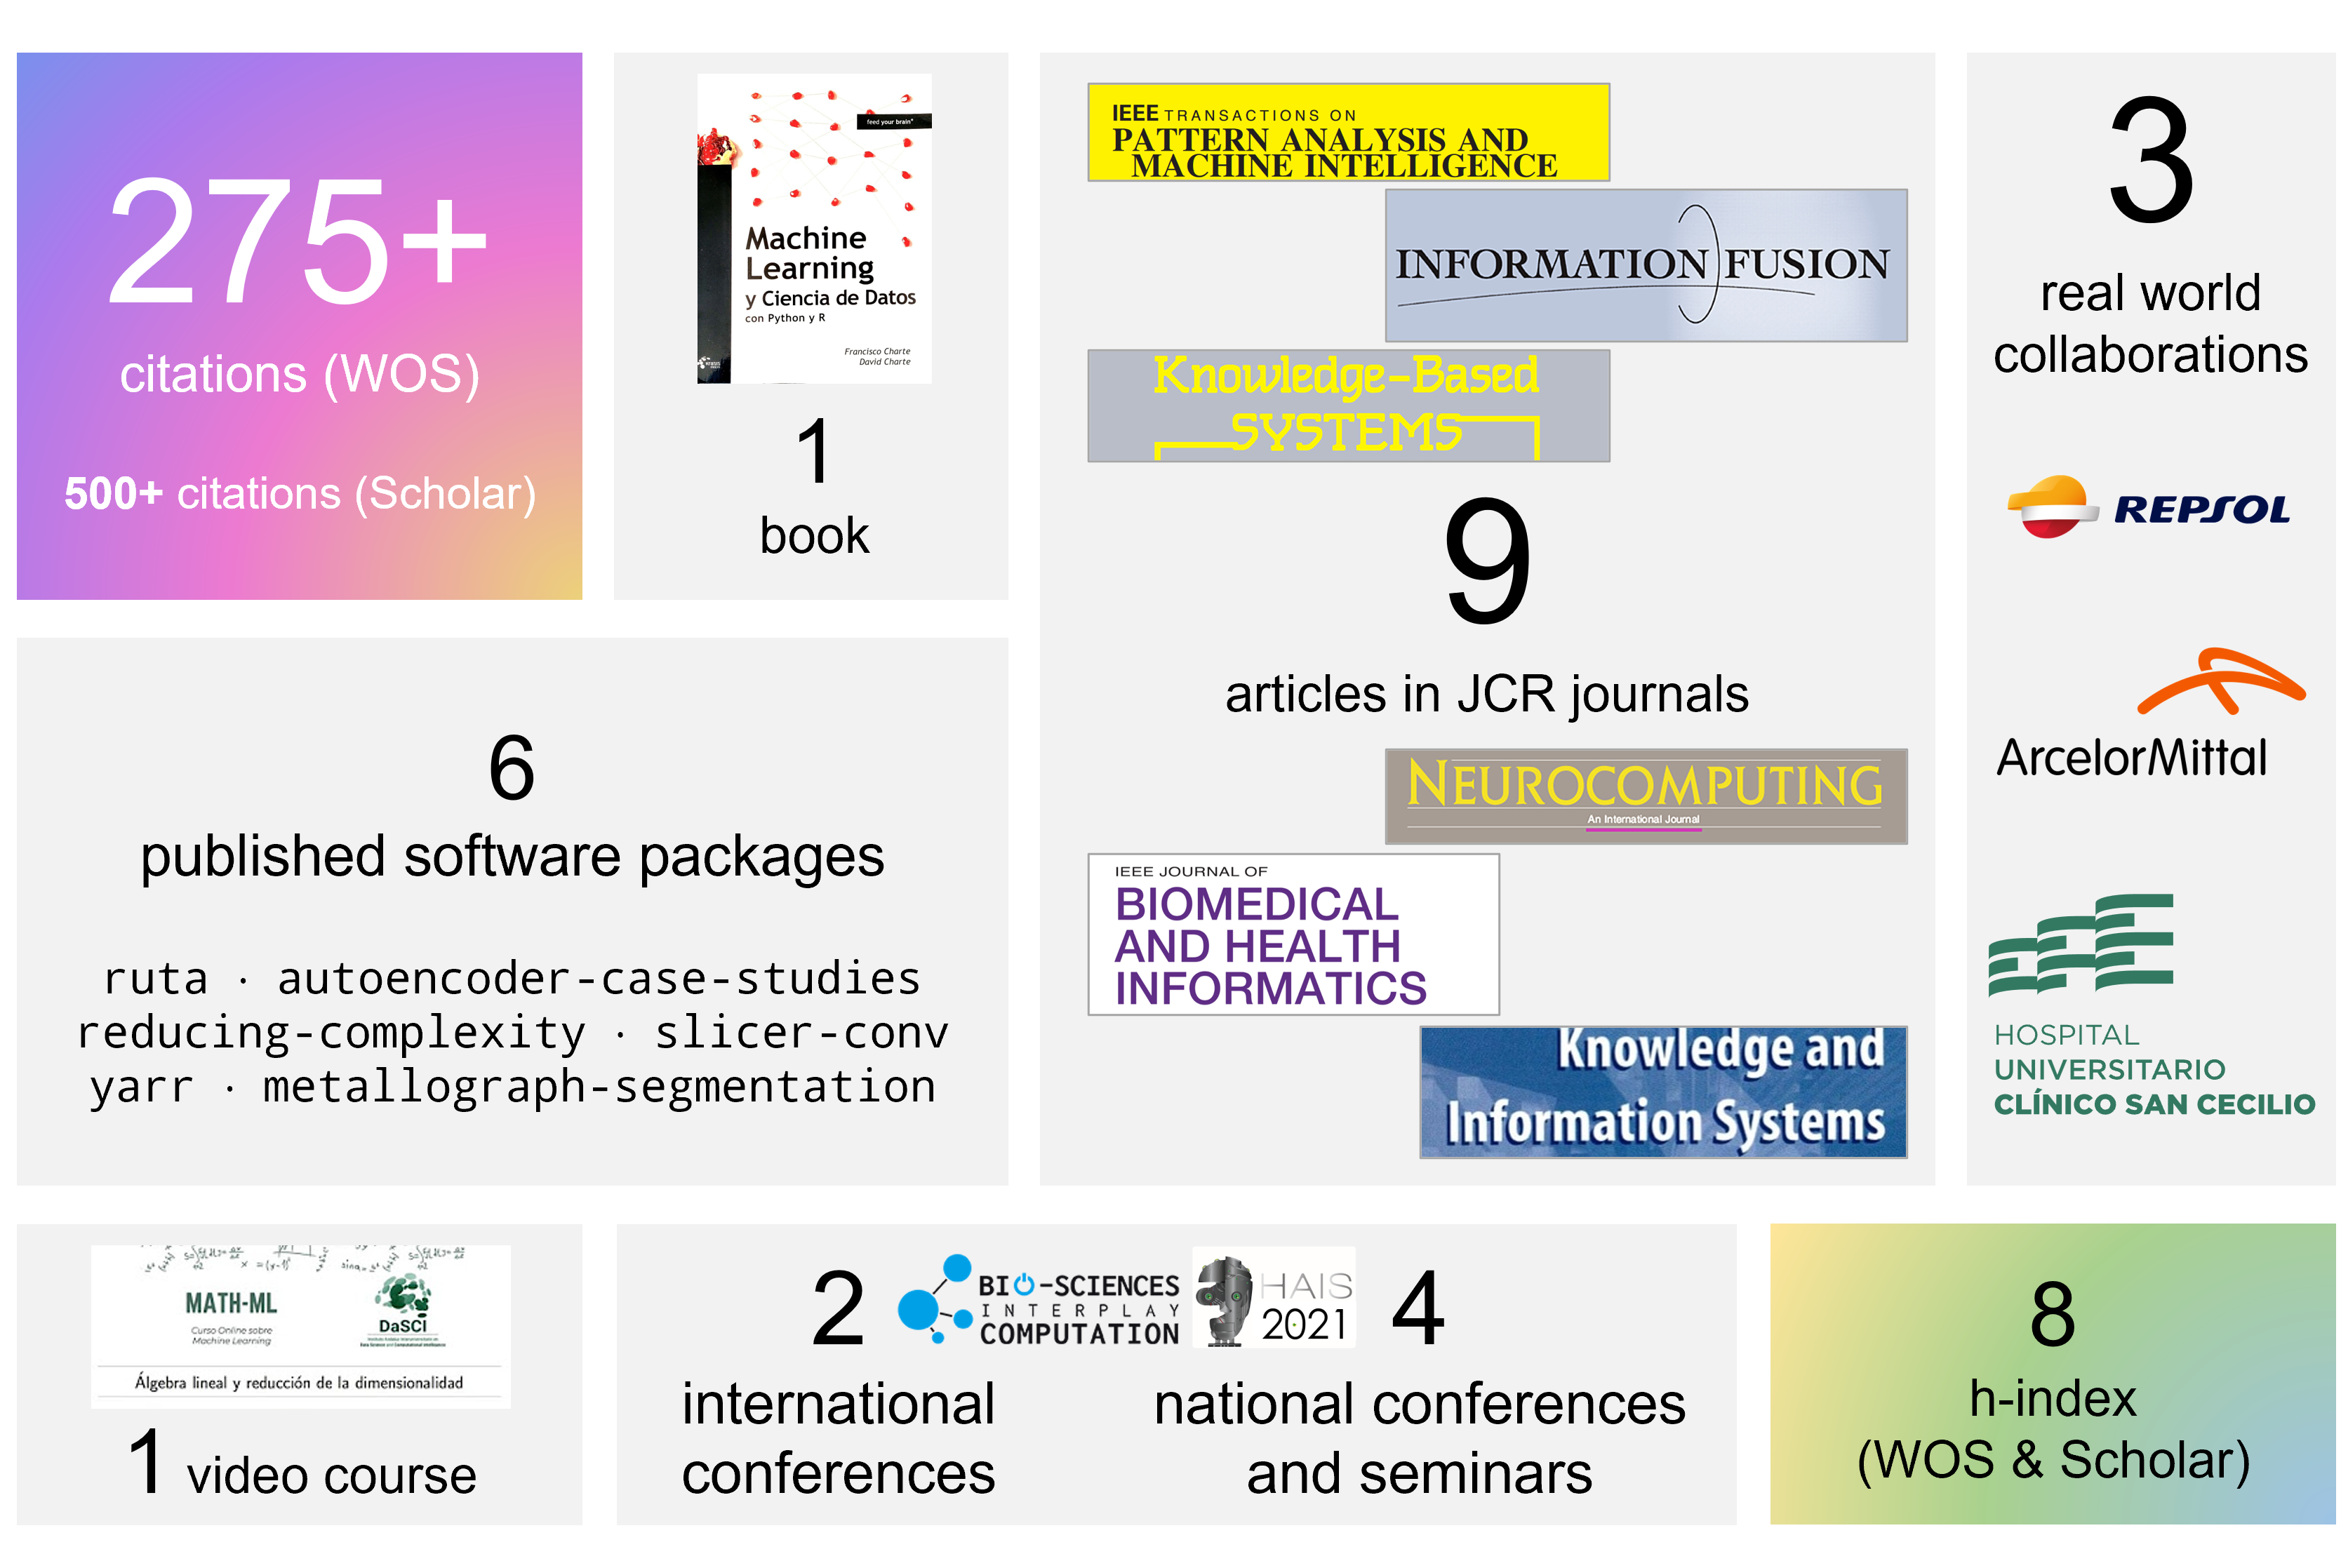
\includegraphics[width=\linewidth]{dashboard}
    \caption{\label{fig:dashboard}Visual summary of the main results obtained during the candidate's research career.}
\end{figure*}

A quick look at the infographic reveals that the focus of this thesis has not only been to produce novel scientific research, but also useful software tools to apply and improve our developments, as well as didactic material which brings this area of computer science closer to different audiences.

In order to not only measure the work by its quantity but also by its impact, mainly within the research community, the joint number of citations through time is shown in \autoref{fig:citations} as well as its position relative to the rest of publications in the same field in \autoref{fig:beamplot}.~

\begin{figure*}[ht!]
    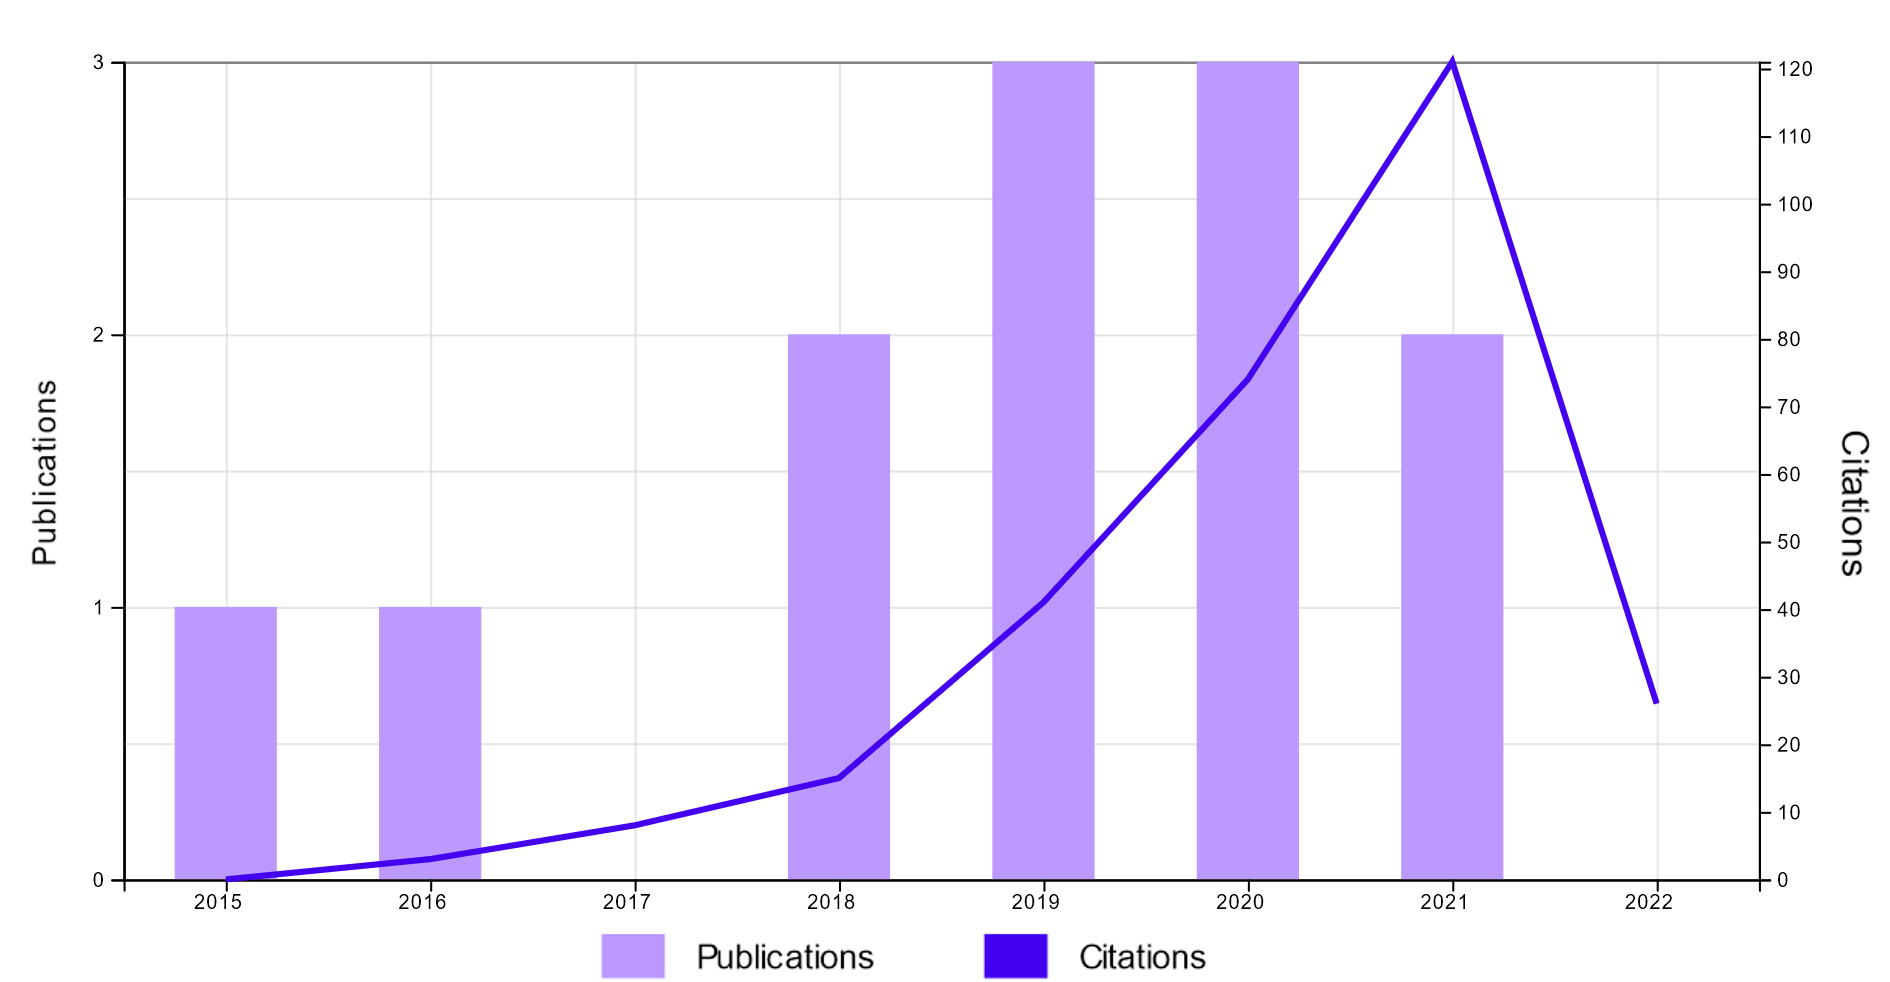
\includegraphics[width=.9\linewidth]{pubs}
    \caption[Graph of the number of publications and citations across years.]{\label{fig:citations}Graph of the number of publications and citations across years (source: Web of Science).}
\end{figure*}
\begin{figure}[hb!]
    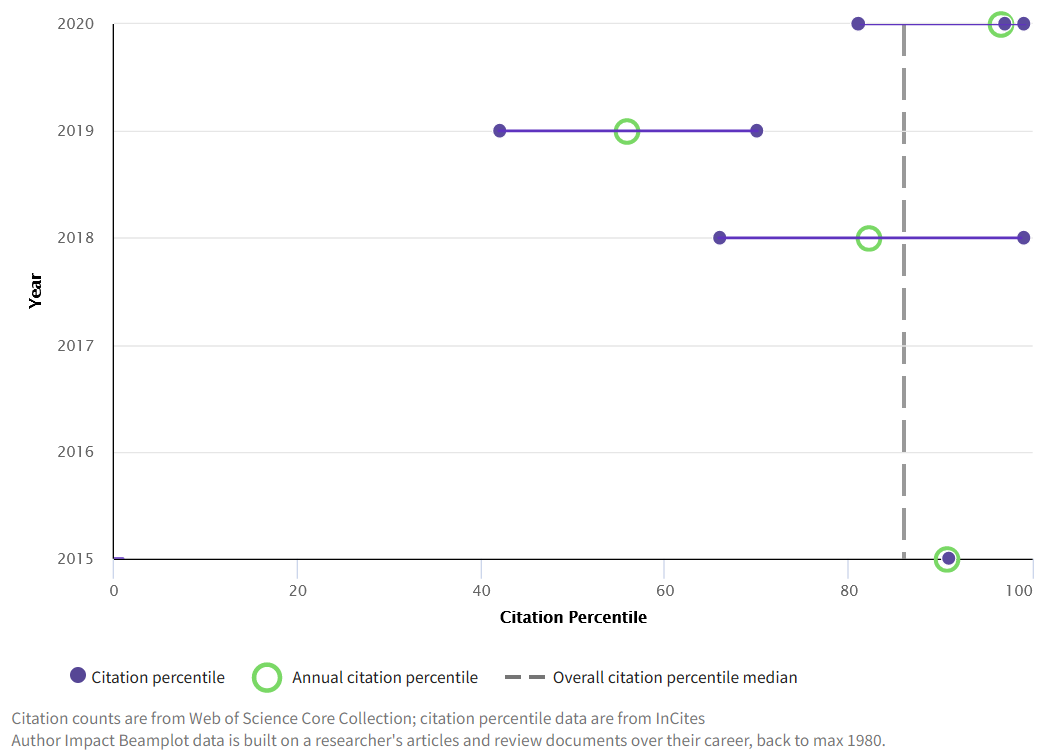
\includegraphics[width=\linewidth]{beamplot}
    \caption[Beamplot displaying the impact of the candidate's publications.]{\label{fig:beamplot}Beamplot displaying the impact of the candidate's publications since 2015 to 2020 (source: Web of Science). Each purple point corresponds to a publication and the horizontal position describes its citation level with respect to the rest of publications in the same area and year (higher is better).}
\end{figure}

\clearpage
\section{Relation of all published material}

The following tables detail all of the candidate's publications as of the time of writing. First, \autoref{tbl:journals} indicates articles published in journals ranked within Journal Citation Reports (JCR), including quality metrics such as journal position in the ranking, quartile and number of citations. 

The rest of publications such as articles in other journals, conference works, talks and one book are broken down in \autoref{tbl:otherpubs}.
\begingroup
\renewcommand{\arraystretch}{1.3}
\begin{table*}[htbp]\scriptsize
    \resizebox{\linewidth}{!}{%
    \begin{tabular}{crp{5.5cm}p{3cm}p{1.6cm}p{0.9cm}rc}
        \toprule
        & \bfseries Year &\bfseries  Title &\bfseries  Journal &\bfseries  Position &\bfseries  Cat. &\bfseries  Cit. &\bfseries  Ref. \\
        \midrule
        & 2015
        &  Working with Multilabel Datasets in R: The mldr Package 
        & The R Journal
        & 56/123 (Q2) & STAT & 30 & \cite{mldr} \\

        & 2018
        &  Tips, guidelines and tools for managing multi-label datasets: The mldr.datasets R package and the Cometa data repository 
        & Neurocomputing
        & 28/134 (Q1) & CS AI & 12 & \cite{cometa} \\

        $\bigstar$ & 2018 
        & A practical tutorial on autoencoders for nonlinear feature fusion: Taxonomy, models, software and guidelines 
        & Information Fusion
        & 
        {2/105 (Q1)\newline 3/134 (Q1)}
        & 
        {CS TM\newline CS AI}
        & 102 & \cite{INFFUS18-AutoencoderTutorial} \\

        $\bigstar$ & 2019 
        & Ruta: Implementations of neural autoencoders in R  
        & Knowledge-based Systems
        & 15/137 (Q1) & CS AI & 4 & \cite{charte2019ruta} \\
        
        $\bigstar$ & 2020 
        &  An analysis on the use of autoencoders for representation learning: Fundamentals, learning task case studies, explainability and challenges 
        & Neurocomputing
        & 30/139 (Q1) & CS AI & 11 & \cite{charte2020analysis} \\

        & 2020 
        &   Artificial intelligence within the interplay between natural and artificial computation: Advances in data science, trends and applications 
        & Neurocomputing
        & 30/139 (Q1) & CS AI & 35 & \cite{interplay} \\

        & 2020 
        &    COVIDGR Dataset and COVID-SDNet Methodology for Predicting COVID-19 Based on Chest X-Ray Images 
        & Biomedical And Health Informatics
        & 28/161 (Q1) & CS IS & 55 & \cite{covid} \\

        & 2021 
        & Revisiting data complexity metrics based on morphology for overlap and imbalance: snapshot, new overlap number of balls metrics and singular problems prospect 
        & Knowledge and Information Systems
        & 65/139 (Q2)$\ast$ & CS AI & 1 & \cite{complexity} \\

        $\bigstar$ & 2021 
        &  Reducing Data Complexity using Autoencoders with Class-informed Loss Functions 
        & Pattern Analysis and Machine Intelligence
        & 1/139 (Q1)$\ast$ & CS AI & n/a & \cite{charte2021reducing} \\

        & 2022 
        &  A tutorial on the segmentation of metallographic images: Taxonomy, new MetalDAM dataset, deep learning-based ensemble model, experimental analysis and challenges 
        & Information Fusion
        & {1/110 (Q1)$\ast$\newline 3/139 (Q1)$\ast$} 
        & {CS TM\newline CS AI} & 0 & \cite{metallography} \\
        \bottomrule
    \end{tabular}}
    \caption[Quality metrics of the articles published in JCR journals during the research period.]{\label{tbl:journals}Quality metrics of the articles published in JCR journals during the research period of the candidate. The position of each journal is taken from the JCR of the corresponding year, except for those marked with an asterisk ($\ast$) which are taken from JCR 2020. The source for the number of citations is Web of Science. Category legends: Statistics and Probability (STAT), Computer Science/Artificial Intelligence (CS AI), Computer Science/Theory and Methods (CS TM), Computer Science/Information Systems (CS IS). Articles marked with a star ($\bigstar$) are part of the core of this thesis.}
\end{table*}

\begin{table*}[htbp]\scriptsize
    \resizebox{\linewidth}{!}{%
    \begin{tabular}{crp{5.5cm}p{2cm}p{4.8cm}c}
        \toprule
        & \bfseries Year &\bfseries  Title &\bfseries  Type &\bfseries  Published in &\bfseries  Ref. \\
        \midrule
        & 2015
        & mldr: Paquete R para exploración de datos multietiqueta
        & National\newline conference
        & XVI Conferencia de la Asociación Española para la Inteligencia Artificial
        & \cite{caepia1} \\

        & 2016
        & Análisis visual de técnicas de \textit{deep learning} no supervisado
        & National\newline conference
        & XVII Conferencia de la Asociación Española para la Inteligencia Artificial
        & \cite{caepia2} \\

        & 2016
        &  R Ultimate Multilabel Dataset Repository 
        & International\newline conference
        & Hybrid Artificial Intelligence Systems
        & \cite{charte2016r} \\

        & 2017
        & Unsupervised Deep Learning in R with Ruta
        & Poster
        & IX Jornadas de usuarios de R
        &  \\

        & 2018
        & A practical tutorial on autoencoders for nonlinear feature fusion: Taxonomy, models, software and guidelines
        & Keywork in\newline national conference
        & XVIII Conferencia de la Asociación Española para la Inteligencia Artificial
        & \cite{caepia3} \\

        $\bigstar$ & 2018
        & A snapshot on nonstandard supervised learning problems: taxonomy, relationships, problem transformations and algorithm adaptations
        & Journal article
        & Progress in Artificial Intelligence (115/171, Q3 in ESCI ranking; Q2 in SJR)
        & \cite{charte2019snapshot} \\

        & 2019
        & A showcase of the use of autoencoders in feature learning applications
        & International\newline conference
        & International Work-Conference on the Interplay between Natural and Artificial Computation
        & \cite{charte2019showcase} \\

        & 2019
        & Aplicaciones prácticas de las redes neuronales no supervisadas
        & National\newline conference
        & Congreso esLibre 2019
        &  \\

        & 2020
        & Autoencoders: An Overview and Applications
        & Talk 
        & Severo Ochoa School on Machine Learning, Big Data, and Deep Learning in Astronomy (IAA-CSIC SOMACHINE)
        &  \\

        & 2021
        & Machine Learning y Ciencia de Datos con Python y R
        & Book
        & Krasis Press
        & \cite{mybook} \\

        & 2021
        & Slicer: Feature Learning for Class Separability with Least-Squares Support Vector Machine Loss and COVID-19 Chest X-Ray Case Study
        & International\newline conference
        & Hybrid Artificial Intelligence Systems
        & \cite{charte2021slicer} \\
        \bottomrule
    \end{tabular}}
    \caption[Other publications, conferences and talks authored by the candidate.]{\label{tbl:otherpubs}Other publications, conferences and talks authored by the candidate. Articles marked with a star ($\bigstar$) are part of the core of this thesis.}
\end{table*}
\endgroup
% \begin{table*}
%     \begin{tabular}[htbp]{lrrrr}
%         \toprule
%         Journal & IF & Q (JIF) & Q (JCI) & Category \\
%         \midrule
%         Pattern Analysis and Machine Intelligence
%         & 16.389 & Q1 & Q1 & CS AI \\
%         Information Fusion
%         & 12.975 & Q1 & Q1 & CS AI \\
%         Knowledge-Based Systems
%         &  8.038 & Q1 & Q1 & CS AI \\
%         Neurocomputing
%         &  5.719 & Q1 & Q1 & CS AI \\
%         Progress in Artificial Intelligence
%         & - & - & Q4 & CS AI \\
%         \midrule
%         Knowledge and Information Systems 
%         &  2.822 & Q2 & Q2 & CS AI, CS IS \\
%         Biomedical and Health Informatics
%         &  5.772 & Q1 & Q1 & CS IS \\
%         \bottomrule
%     \end{tabular}
%     \caption{\label{tbl:journals}Quality metrics of the journals where articles have been coauthored by the candidate during the course of the thesis. Columns indicate the impact factor (IF) and the quartile according to Journal Impact Factor (JIF) and Journal Citation Indicator (JCI).}
% \end{table*}

\clearpage
\section{Main articles}

From the works previously mentioned, five peer-review articles have been selected as the main core of this thesis for advancing our fundamental objectives.

The first objective, as described previously in Section~\ref{sec:objectives}, was to study autoencoders and contribute to more people being able to use them to solve their tasks. Article~\ref{ch:paper1} \sidecite{INFFUS18-AutoencoderTutorial} addresses this by describing autoencoder fundamentals, its variants, implementations and providing tips on autoencoder design depending on the problem at hand.

Continuing with the objective of facilitating access to autoencoders, Article~\ref{ch:paper2} \sidecite{charte2019ruta} presents Ruta, a software library which simplifies the creation and training process. It is programmed in the R language to ease the transition from other tools for users with little programming knowledge.

Next, part of the time was devoted to exploring a diverse range of problems where autoencoders could be applicable. Article~\ref{ch:paper3} \sidecite{charte2019snapshot} organizes the knowledge around a variety of supervised problems, for example, multi-instance classification and multi-output regression. For its part, Article~\ref{ch:paper5} \sidecite{charte2020analysis} analyzes another list of problems, mostly unsupervised, where autoencoder-based models have already been applied as a valid solution, from anomaly detection to instance generation.

Some preliminary work was accomplished into approaching one of the nonstandard supervised problems, label distribution learning, using an autoencoder-based solution. This did not improve on current, simpler techniques so our focus changed onto tackling a more general situation that could be then applied to multiple supervised problems. This new development, consisting of a model which is able to extract features with better class separability than most traditional feature learners, is detailed in Article~\ref{ch:paper6} \sidecite{charte2021reducing}. We also demonstrate the usefulness of this novel solution by applying it to a specific problem, detection of COVID-related pulmonar symptoms in X-ray images, in \sidecite{charte2021slicer}.
